\documentclass[11pt]{article}
\usepackage[paperheight=15in, left=2cm, right=2cm, top=2cm, bottom=2cm]{geometry}
\usepackage[most]{tcolorbox}
\usepackage{amsmath, amssymb, amsthm, enumitem, stmaryrd, cancel, pifont, dsfont, hyperref, fancyhdr, lastpage, tocloft, changepage, tkz-tab, tikz-among-us}

\newcommand*{\K}{\mathbb{K}}
\newcommand*{\C}{\mathbb{C}}
\newcommand*{\R}{\mathbb{R}}
\newcommand*{\Q}{\mathbb{Q}}
\newcommand*{\Z}{\mathbb{Z}}
\newcommand*{\N}{\mathbb{N}}
\newcommand*{\F}{\mathcal{F}}
\newcommand*{\CM}{\mathcal{CM}}
\newcommand*{\m}{\mathcal}

\newcommand{\0}{\varnothing}
\newcommand*{\e}{\varepsilon}
\newcommand*{\g}{\gamma}
\newcommand*{\s}{\sigma}
\renewcommand*{\l}{\lambda}
\renewcommand*{\t}{\tau}

\newcommand*{\ra}{\Longrightarrow}
\newcommand*{\la}{\Longleftarrow}
\newcommand*{\rla}{\Longleftrightarrow}
\newcommand*{\lb}{\llbracket}
\newcommand*{\rb}{\rrbracket}
\newcommand*{\n}{\\[0.2cm]}

\newcommand*{\cmark}{\ding{51}}
\newcommand*{\xmark}{\ding{55}}

\newcommand{\dx}{\textrm{d}x}
\newcommand{\dt}{\textrm{d}t}
\newcommand{\rg}[1]{\textrm{rg}(#1)}
\newcommand{\vect}[1]{\textrm{Vect}(#1)}
\newcommand{\tr}[1]{\textrm{Tr}(#1)}

\renewcommand*{\Re}{\textrm{Re}}
\renewcommand{\dim}[1]{\textrm{dim}~#1}
\renewcommand*{\ker}[1]{\textrm{Ker}(#1)}
\renewcommand{\Im}{\textrm{Im}}
\renewcommand*{\phi}{\varphi}

\newcommand{\providetcbcountername}[1]{%
  \@ifundefined{c@tcb@cnt@#1}{%
    --undefined--%
  }{%
    tcb@cnt@#1%
  }
}

\newcommand{\settcbcounter}[2]{%
  \@ifundefined{c@tcb@cnt@#1}{%
    \GenericError{Error}{counter name #1 is no tcb counter }{}{}%
  }{%
    \setcounter{tcb@cnt@#1}{#2}%
   }%
}%

\newcommand{\displaytcbcounter}[1]{% Wrapper for \the...
  \@ifundefined{thetcb@cnt@#1}{%
    \GenericError{Error}{counter name #1 is no tcb counter }{}{}%
  }{%
    \csname thetcb@cnt@#1\endcsname% 
  }%
}

% MATHS %
\newtcbtheorem{thm}{Théorème}
{
    enhanced,frame empty,interior empty,
    colframe=red,
    after skip = 1cm,
    borderline west={1pt}{0pt}{green!25!red},
    borderline south={1pt}{0pt}{green!25!red},
    left=0.2cm,
    attach boxed title to top left={yshift=-2mm,xshift=-2mm},
    coltitle=black,
    fonttitle=\bfseries,
    colbacktitle=white,
    boxed title style={boxrule=.4pt,sharp corners},
    before lower = {\textbf{Preuve :}\n}
}{thm}

\newtcbtheorem[use counter from = thm]{defi}{Définition}
{
    enhanced,frame empty,interior empty,
    colframe=green,
    after skip = 1cm,
    borderline west={1pt}{0pt}{green},
    borderline south={1pt}{0pt}{green},
    left=0.2cm,
    attach boxed title to top left={yshift=-2mm,xshift=-2mm},
    coltitle=black,
    fonttitle=\bfseries,
    colbacktitle=white,
    boxed title style={boxrule=.4pt,sharp corners},
    before lower = {\textbf{Preuve :}\n}
}{defi}

\newtcbtheorem[use counter from = thm]{prop}{Proposition}
{
    enhanced,frame empty,interior empty,
    colframe=blue,
    after skip = 1cm,
    borderline west={1pt}{0pt}{green!25!blue},
    borderline south={1pt}{0pt}{green!25!blue},
    left=0.2cm,
    attach boxed title to top left={yshift=-2mm,xshift=-2mm},
    coltitle=black,
    fonttitle=\bfseries,
    colbacktitle=white,
    boxed title style={boxrule=.4pt,sharp corners},
    before lower = {\textbf{Preuve :}\n}
}{prop}

\newtcbtheorem[use counter from = thm]{corr}{Corrolaire}
{
    enhanced,frame empty,interior empty,
    colframe=blue,
    after skip = 1cm,
    borderline west={1pt}{0pt}{green!25!blue},
    borderline south={1pt}{0pt}{green!25!blue},
    left=0.2cm,
    attach boxed title to top left={yshift=-2mm,xshift=-2mm},
    coltitle=black,
    fonttitle=\bfseries,
    colbacktitle=white,
    boxed title style={boxrule=.4pt,sharp corners},
    before lower = {\textbf{Preuve :}\n}
}{corr}

\newtcbtheorem[use counter from = thm]{lem}{Lemme}
{
    enhanced,frame empty,interior empty,
    colframe=blue,
    after skip = 1cm,
    borderline west={1pt}{0pt}{green!25!blue},
    borderline south={1pt}{0pt}{green!25!blue},
    left=0.2cm,
    attach boxed title to top left={yshift=-2mm,xshift=-2mm},
    coltitle=black,
    fonttitle=\bfseries,
    colbacktitle=white,
    boxed title style={boxrule=.4pt,sharp corners},
    before lower = {\textbf{Preuve :}\n}
}{lem}

\newtcbtheorem[use counter from = thm]{ex}{Exemple}
{
    enhanced,frame empty,interior empty,
    colframe=orange,
    after skip = 1cm,
    borderline west={1pt}{0pt}{orange},
    borderline south={1pt}{0pt}{orange},
    left=0.2cm,
    attach boxed title to top left={yshift=-2mm,xshift=-2mm},
    coltitle=black,
    fonttitle=\bfseries,
    colbacktitle=white,
    boxed title style={boxrule=.4pt,sharp corners},
    before lower = {\textbf{Preuve :}\n}
}{ex}

\newtcbtheorem[use counter from = thm]{meth}{Méthode}
{
    enhanced,frame empty,interior empty,
    colframe=purple,
    after skip = 1cm,
    borderline west={1pt}{0pt}{purple},
    borderline south={1pt}{0pt}{purple},
    left=0.2cm,
    attach boxed title to top left={yshift=-2mm,xshift=-2mm},
    coltitle=black,
    fonttitle=\bfseries,
    colbacktitle=white,
    boxed title style={boxrule=.4pt,sharp corners},
    before lower = {\textbf{Preuve :}\n}
}{meth}

% PHYSIQUE %
\newtcbtheorem[use counter from = thm]{qc}{Question de Cours}
{
    enhanced,frame empty,interior empty,
    colframe=red,
    after skip = 1cm,
    borderline west={1pt}{0pt}{green!25!red},
    borderline south={1pt}{0pt}{green!25!red},
    left=0.2cm,
    attach boxed title to top left={yshift=-2mm,xshift=-2mm},
    coltitle=black,
    fonttitle=\bfseries,
    colbacktitle=white,
    boxed title style={boxrule=.4pt,sharp corners},
    before lower = {\textbf{Preuve :}\n}
}{qc}
\newtcbtheorem[use counter from = thm]{app}{Application}
{
    enhanced,frame empty,interior empty,
    colframe=blue,
    after skip = 1cm,
    borderline west={1pt}{0pt}{green!25!blue},
    borderline south={1pt}{0pt}{green!25!blue},
    left=0.2cm,
    attach boxed title to top left={yshift=-2mm,xshift=-2mm},
    coltitle=black,
    fonttitle=\bfseries,
    colbacktitle=white,
    boxed title style={boxrule=.4pt,sharp corners},
    before lower = {\textbf{Preuve :}\n}
}{app}

\def\pagetitle{Intégrales sur un segment}
\setlength{\headheight}{14pt}

\title{\bf{\pagetitle}\n\large{Corrigé}}

\hypersetup{
    colorlinks=true,
    citecolor=black,
    linktoc=all,
    linkcolor=blue
}

\pagestyle{fancy}
\cfoot{\thepage\ sur \pageref*{LastPage}}

\begin{document}

\thispagestyle{fancy}
\fancyhead[L]{MP2I Paul Valéry}
\fancyhead[C]{\pagetitle}
\fancyhead[R]{2023-2024}

\hrule
\begin{center}
    \LARGE{\textbf{Chapitre 35}}\n
    \large{\pagetitle}\n
    \rule{0.8\textwidth}{0.5pt}
\end{center}


\vspace{0.5cm}

\section{Intégrale d'une fonction continue sur un segment}
\subsection{Ensemble $\CM(I,\K)$}

\begin{defi}{Fonction continue par morceaux sur un intervalle.}{}
    Soit $I$ un intervalle et $f:I\to\K$. On dit que $f$ est \textbf{continue par morceaux} sur $I$ si pour tout segment $[a,b]\subset I$, $f_{|[a,b]}$ est continue par morceaux sur $[a,b]$.\\
    On note $\CM(I,\K)$ l'ensemble des fonctions continues par morceaux sur $I$.
\end{defi}

\begin{ex}{$x\mapsto\lfloor\frac{1}{x}\rfloor$}{}
La fonction $x\mapsto\lfloor\frac{1}{x}\rfloor$ est continue par morceaux sur $\R^*_+$. Expliquer.
\tcblower
Soit $[a,b]\subset\R^*_+$. Notons $S=\{\frac{1}{n}\mid n\in\N^*\}\cap]a,b[$.\\
Cet ensemble est finito : pour $n\in\N^*$, $a<\frac{1}{n}<b\iff\frac{1}{b}<n<\frac{1}{a}\iff\lfloor\frac{1}{b}\rfloor+1 \leq n \leq \lfloor\frac{1}{a}\rfloor$.\\
$S$ contient donc au plus $\lfloor\frac{1}{a}\rfloor-\lfloor\frac{1}{b}\rfloor$ points.\\
Notons $n=|S|$ puis $S=\{a_1,...,a_n\}$, avec $a_1<a_2<...<a_n$.\\
Posons $\s=(a_0,a_1,...,a_n,a_{n+1})$ avec $a_0 := a$ et $a_{n+1} := b$.\\
Soit $i\in\lb0,\rb$, $f_{|]a_i,a_{i+1}[}$ est constante, elle y est donc continue et prolongeable par continuité aux bords.
Ainsi, $f\in\CM(\R^*_+,\R)$.\\
\textbf{Remarque:} En posant $f(0):=0$, ça ne marche plus car $f_{|[0,b]}$ n'est pas cpm sur $[0,b]$.
\end{ex}

\subsection{Intégrale d'une fonction continue par morceaux entre deux bornes}
\begin{defi}{}{}
    Soit $f\in\CM(I,\R)$ et $a,b\in I$. On note $\int_a^bf(x)\dx$, ou plus simplement $\int_a^bf$ le réel défini par :
    \begin{equation*}
        \int_a^bf(x)\dx:=\int_{[a,b]}f ~ \text{si} ~ a<b, \quad \int_a^af(x)\dx:=0,\quad \text{et}\quad\int_a^bf(x)\dx:=-\int_{[b,a]}f~\text{si } a>b.
    \end{equation*}
\end{defi}

\begin{prop}{}{}
    Soit $f\in\CM(I,\C)$.\\
    Les fonctions $x\mapsto\Re(f(x))$ et $x\mapsto\Im(f(x))$ sont continues par morceaux sur $I$.\\
    Pour $a,b\in I$, on pose :
    \begin{equation*}
        \int_a^bf(x)\dx:=\int_a^b\Re(f(x))\dx+i\int_a^b\Im(f(x))\dx.
    \end{equation*}
    Ainsi, la partie réelle de l'intégrale est l'intégrale de la partie réelle, idem pour la partie imaginaire.
    \tcblower
    Pour prouver la continuité par morceaux de $\Re(f)$ et $\Im(f)$ à partir de celle de $f$, on introduit une subdivision adaptée à $f$ $\s=(a_0,...,a_n)$ et on prouve qu'elle est adaptée à sa partie réelle et à sa partie imaginaire. On peut utiliser :
    \begin{equation*}
        \forall x\in I ~ \Re(f(x)) = \frac{1}{2}(f(x)+\overline{f(x)}) ~ \text{et} ~ \Im(f(x))=\frac{1}{2i}(f(x)-\overline{f(x)}).
    \end{equation*}
    En effet, ces relations donnent que pour $i\in\lb0,n-1\rb$, les restrictions de $\Re(f)$ et $\Im(f)$ à $]a_i,a_{i+1}[$ y sont continues, et prolongeables par continuité sur les bords.
\end{prop}

\pagebreak
\subsection{Relation de Chasles.}
\begin{prop}{Relation de Chasles}{}
    Soient $f\in\CM(I,\K)$ et $a,b,c\in I$.
    \begin{equation*}
        \int_a^bf=\int_a^cf+\int_c^bf.
    \end{equation*}
    \tcblower
    La relation a été établie dans le cours de construction pour une fonction à valeurs réelles dans le cas où $a<c<b$.\\
    $\bullet$ cas $a<b<c$ :
    \begin{equation*}
        \int_a^cf+\int_c^bf=\int_{[a,c]}f-\int_{[b,c]}f=\int_{[a,b]}f+\int_{[b,c]}f-\int_{[b,c]}f=\int_{[a,b]}f=\int_a^bf.
    \end{equation*}
    $\bullet$ cas $b=c<a$ :\\
    D'une part $\int_a^bf=-\int_{[b,a]}f$, d'autre part : $\int_a^cf+\int_c^bf=-\int_c^af=-\int_[b,a]f$.\n
    Les autres cas sont similaires.
\end{prop}

\subsection{Linéarité.}

\begin{prop}{Linéarité de l'intégrale.}{}
    Soient $f,g\in\CM(I,\K)$, et $a,b\in I$. Pour tous scalaires $\l,\mu\in\K$,
    \begin{equation*}
        \int_a^b(\l f+\mu g) = \l\int_{a}^bf+\mu\int_a^bg.
    \end{equation*}
    \tcblower
    On l'a prouvé pour $a<b$ et $f,g$ à valeurs réelles. Il faut le vérifier dans les autres cas.
\end{prop}

\subsection{Intégrales et inégalités.}
\begin{prop}{Positivité}{}
    Soit $f\in\CM([a,b],\R)$ où le segment $[a,b]$ est tel que \fbox{$a\leq b$}.\\
    Si $f$ est positive sur $[a,b]$, alors l'intégrale $\int_a^bf(x)\dx$ est un nombre positif.\\
    Si $f$ est négative sur $[a,b]$, alors cette intégrale est un nombre négatif.
    \tcblower
    On l'a déjà prouvé.
\end{prop}

\begin{prop}{Intégrale nulle d'une fonction positive et continue}{}
    Soit $f:[a,b]\to\R$, avec \fbox{$a<b$}, continue et positive sur $[a,b]$.\\
    Si $\int_a^bf(x)\dx=0$, alors $f$ est nulle sur $[a,b]$.\\
    Par contraposée, si $\exists c \in [a,b] ~ f(c)>0$, alors $\int_a^bf>0$.
    \tcblower
    Il y a aussi la preuve suivante dans \textbf{L'Exercice 79} de la banque CCINP :\\
    On suppose $f$ continue et positive sur $[a,b]$ et $\int_a^bf=0$.\\
    Posons $F:x\mapsto\int_a^xf(t)\dt$ définie sur $[a,b]$, $f$ étant continue sur $[a,b]$, $F$ est une primitive de $f$ sur $[a,b]$ d'après le TFA (prouvé plus loin).\\
    Donc $\forall x \in [a,b], ~ F'(x)=f(x)\geq0$, ainsi $F$ est croissante sur $[a,b]$.\\
    Or, $F(b)=\int_a^bf=0$, de plus, $F(a)=\int_a^af=0$.\\
    Par croissance, $\forall x \in [a,b], ~ F(a) \leq F(x)\leq F(b)$ donc $F(x)=0$.\\
    Donc $F$ est constante sur $[a,b]$, on a $a<b$ donc $\forall x\in[a,b], ~ F'(x)=f(x)=0$.
    \n\textbf{Remarque:} Pourquoi continue et pas continue par morceaux ?\\
    Soit $f:\begin{cases}[0,1]\to\R\\x\mapsto\begin{cases}0 \text{ si } x\neq\frac{1}{2}\\1 \text{ si } x=\frac{1}{2}\end{cases}\end{cases}$, son intégrale est nulle, mais $f$ ne l'est pas.
\end{prop}

\begin{prop}{Croissance}{}
    Soient $f,g\in\CM([a,b],\R)$ avec \fbox{$a\leq b$}.
    \begin{equation*}
        f \leq g ~ \Longrightarrow ~ \int_a^bf(x)\dx \leq \int_a^b g(x)\dx
    \end{equation*}
    \tcblower
    On a :
    \begin{equation*}
        \int_a^b g - \int_a^b f = \int_a^b(g-f)
    \end{equation*}
    Comme $g-f$ est continue par morceaux et positive, on a $\int_a^b(g-f)\geq0$ donc $\int_a^bf\leq\int_a^bg$.
\end{prop}

\begin{prop}{Inégalité de la moyenne}{}
    Soit $f\in\CM([a,b], \R)$ avec \fbox{$a\leq b$}.\\
    Si $f$ est minorée par un réel $m$ et majorée par $M$ sur $[a,b]$, alors :
    \begin{equation*}
        m(b-a) \leq \int_a^bf(x)\dx \leq M(b-a),~\text{Lorsque }a<b, \text{ on a } m\leq\frac{1}{b-a}\int_a^bf(x)\dx\leq M.
    \end{equation*}
    \tcblower
    On a $\forall x\in[a,b], ~ m \leq f(x) \leq M$.\\
    La fonction $f$, $x\mapsto m$, $x\mapsto M$ sont continues par morceaux.\\
    Par croissance :
    \begin{equation*}
        \int_a^bm\dt\leq \int_a^bf(t)\dt\leq\int_a^bM\dt
    \end{equation*}
    Donc
    \begin{equation*}
        m(b-a) \leq \int_a^bf(t)\dt\leq M(b-a)
    \end{equation*}
\end{prop}

\begin{prop}{Inégalité triangulaire}{}
    Soit $f\in\CM([a,b], \K)$, avec \fbox{$a\leq b$}.
    \begin{equation*}
        \left|\int_a^bf(x)\dx\right|\leq\int_a^b|f(x)|\dx
    \end{equation*}
    \tcblower
    $\circledcirc$ \textbf{Cas réel:} Soit $f\in\CM([a,b], \R)$.\\
    On a $f\leq|f|$ et $-f\leq|f|$, or $f, -f$ et $|f|$ sont cpm sur $[a,b]$.\\
    Par croissance de l'intégrale ($a\leq b$) : $\int_a^b f \leq \int_a^b|f|$ et $-\int_a^bf \leq\int_a^b|f|$.\\
    Donc $\max(\int_a^b f, -\int_a^b f) \leq \int_a^b|f|$ et alors $\left|\int_a^b f\right|\leq\int_a^b|f|$.\\
    $\circledcirc$ \textbf{Cas complexe:} admis.
\end{prop}

\subsection{Quelques exercices de cours.}

\begin{ex}{}{}
    Pour $a\in\R^*_+$, on pose $I_a=\int_a^{a^2}\ln^3(x)\dx$. Existence et signe de $I_a$.
    \tcblower
    \textbf{Existence:} $\ln^3$ est continue (par morceaux) sur $\R^*_+$.\\
    \textbf{1er cas:} Supposons $a\geq1$, alors $a\leq a^2$ et $\forall x \in [a,a^2] ~ \ln^3(x) \geq 0$, par positivité, $\int_a^{a^2}\ln^3\geq0$.\\
    \textbf{2eme cas:} Supposons $a\in]0,1[$, alors $a^2\leq a$ et $\forall x \in [a^2, a] ~ \ln^3(x)\leq0$, par positivité, $\int_{a^2}^a\ln^3\leq0$ donc $\int_a^{a^2}\ln^3\geq0$.\\
    Ainsi, $\forall a\in\R^*_+, ~ I_a\geq0$
\end{ex}

\begin{ex}{}{}
    Soit $f:[a,b]\to\R$ avec $a<b$ continue telle que $\int_a^bf(t)\dt=0$.\\
    Justifier que $f$ s'annule au moins une fois sur $[a,b]$.
    \tcblower
    \textbf{1er cas:} Supposons que $f$ change de signe sur $[a,b]$, alors d'après le TVI, $f$ s'annule sur $[a,b]$ puisque $f$ est continue.\\
    \textbf{2eme cas:} Supposons que $f$ ne change pas de signe sur $[a,b]$. On a que $a<b$, que $f$ est continue et monotone sur $[a,b]$, et d'intégrale nulle. Par théorème, $\forall x \in [a,b], ~ f(x)=0$.\n
    On peut aussi le prouver avec le TFA + Rolle.
\end{ex}

\begin{ex}{Un exercice : suite définie par une intégrale.}{}
    Soit, pour $n\in\N, I_n := \int_1^e(\ln(x))^n\dx$.\\
    \-\ ~1. Prouver que $(I_n)$ est convergente.\\
    \-\ ~2. Prouver que la limite vaut 0 à l'aide d'une IPP.\\
    \-\ ~3. Donner un équivalent de $I_n$.
    \tcblower
    \boxed{1.} \textbf{Monotonie:} Soit $n\in\N$.
    \begin{equation*}
        I_{n+1} - I_n = \int_1^e\underbrace{(\ln(x))^n}_{\geq0}\underbrace{(\ln(x)-1)}_{\leq0}\dx
    \end{equation*}
    La fonction $x\mapsto (\ln(x))^n(\ln(x)-1)$ est continue sur $[1,e]$ on a $1\leq e$ et la fonction est négative.\\
    Par positivité de l'intégrale, $I_{n+1}-I_n\leq0$ et donc $(I_n)$ est décroissante.\\
    \textbf{Convergence:} Par positivité, on a $\forall n \in \N, ~ I_n \geq 0$, donc $I_n$ est décroissante et minorée par $0$ donc elle converge d'après le TLM.\\
    \boxed{2.} Une IPP pour trouver une relation de récurrence. Pour $n\in \N^*$ :
    \begin{align*}
        I_n &= \int_1^e(\ln(x))^n\dx\\&=\left[ x(\ln(x))^n \right]_1^e - \int_1^e\cancel{x}n\cancel{\frac{1}{x}}(\ln(x))^{n-1}\dx\\&=e-nI_{n-1}
    \end{align*}
    On a $\forall n \in \N^* ~ I_{n} = \frac{1}{n+1}(e-I_{n+1})$. Notons $l=\lim I_n$, qui existe d'après \boxed{1.}.\\
    Alors $I_n = \frac{1}{n+1}(e-I_{n+1})\to0$ car $e-I_{n+1}\to e - l$.\\
    \boxed{3.} On a $nI_n = \frac{n}{n+1}(e-I_{n+1})\to e$ donc $I_n \sim \frac{e}{n}$.
\end{ex}

\begin{ex}{Lemme de Riemann-Lebesgue}{}
    Soit $f\in\m{C}^1([a,b],\C)$. Montrer que
    \begin{equation*}
        \int_a^bf(t)e^{int}\dt\to0.
    \end{equation*}
    \textbf{Remarque:} Le lemme est vrai pour $f$ continue sur $[a,b]$, mais difficile à démontrer.
    \tcblower
    Idée : IPP. Soit $n\in\N$. $f$ et $\frac{1}{in}e^{int}$ sont de classe $\m{C}^1$ sur $[a,b]$ donc :
    \begin{equation*}
        \int_a^bf(t)e^{int}\dt=\left[ f(t)\cdot\frac{1}{in}e^{int} \right]_a^b - \int_a^b f'(t)\cdot\frac{1}{in}e^{int}\dt
    \end{equation*}
    Alors
    \begin{align*}
        |I_n|=\Big|...\Big|\leq \Big|[...]_a^b\Big| + \Big|\int_a^b...\Big|
    \end{align*}
    D'une part : $\Big|\left[ f(t)\frac{1}{in} e^{int}\right]_a^b\Big|=\frac{1}{n}\Big|f(b)e^{inb}-f(a)e^{ina}\Big|\leq\frac{1}{n}(|f(b)|+|f(a)|)$.\\
    D'autre part : $\Big|\int_a^bf'(t)\frac{1}{in}e^{int}\dt\Big|\leq\frac{1}{n}\int_a^b\Big|f'(t)\Big|\dt$.\\
    Par majoration, $|I_n|=O(\frac{1}{n})$ donc $I_n\to0$.
\end{ex}

\begin{thm}{Théorème fondamental de l'analyse}{}
    Soit $I$ un intervalle et $f:I\to\K$ une fonction continue sur $I$. Soit $a\in I$. La fonction
    \begin{equation*}
        E: \begin{cases}
           I~\to~\K\\
           x~\mapsto~F(x) = \int_a^xf(t)\dt 
        \end{cases}
    \end{equation*}
    est de classe $\m{C}^1$ sur $I$ et de dérivée $F'=f$.
    \tcblower
    Soit $x_0\in I$. Montrons que $\frac{F(x)-F(x_0)}{x-x_0}\to f(x_0)$\\
    Soit $x\in I\setminus\{x_0\}$.
    \begin{align*}
        \left|\frac{F(x)-F(x_0)}{x-x_0}-f(x_0)\right|&=\left|\frac{1}{x-x_0}\left(\int_a^xf(t)\dt-\int_a^{x_0}f(t)\dt\right)-f(x_0)\right|\\
        &=\left|\frac{1}{x-x_0}\int_{x_0}^xf(t)\dt-\frac{1}{x-x_0}\int_{x_0}^xf(x_0)\dt\right|\\
        &=\frac{1}{|x-x_0|}\left|\int_{x_0}^x(f(t)-f(x_0))\dt\right|\\
        &\leq\frac{1}{|x-x_0|}\int_{\min(x_0,x)}^{\max(x_0,x)}\left|f(t)-f(x_0)\right|\dt
    \end{align*}
    Soit $\e>0$. Par continuité de $f$ en $x_0$, $\exists \eta>0 \forall x \in I\cap]x_0-\eta,x_0+\eta[~|f(t)-f(x_0)|\leq\e$.\\
    Supposons que $|x-x_0|\leq\eta$. Alors $[\min(x_0,x), \max(x_0,x)]\subset I\cap]x_0-\eta,x_0+\eta[$.\\
    Par croissance :
    \begin{equation*}
        \int_{\min}^{\max}\Big|f(t)-f(x_0)\Big|\dt\leq\int_{\min}^{\max}\e\dt = \e(\max - \min) = \e|x-x_0|.
    \end{equation*}
    Ainsi, $\Big|\frac{F(x)-F(x_0)}{x-x_0}-f(x_0)\Big|\leq\frac{1}{|x-x_0|}\e|x-x_0|=\e$
\end{thm}

\begin{corr}{}{}
    Toute fonction continue sur un intervalle y admet des primitives.\\
    Sur un intervalle, deux primitives d'une même fonction diffèrent d'une constante.
    \tcblower
    Le TFA donne bien une primitive sous ces hypothèses.\\
    Soit $f\in\m{C}(I,\K)$, $F$ et $G$ deux primitives de $f$.\\
    Alors $F-G$ est dérivable sur $I$ et $(F-G)'=f-f=0$ donc $F-G$ est constante sur $I$ d'après AF.
\end{corr}

\begin{prop}{}{}
    Soit $f\in\m{C}(I,\K)$ et $F$ une primitive de $f$ sur $I$. Alors, pour tous $a,b\in I$,
    \begin{equation*}
        \int_a^bf(t)\dt=F(b)-F(a)
    \end{equation*}
    \tcblower
    On a $f$ continue sur $[a,b]$. Le TFA donne $\tilde{F}:x\mapsto\int_a^xf(t)\dt$ primitive de $f$ sur $[a,b]$.\\
    La fonction $F$ en est une autre, sur le même intervalle : $\exists C\in\K ~ \forall x \in [a,b] ~ \tilde{F}(x)=F(x)+C$.\\
    Alors :
    \begin{equation*}
        \int_a^bf(t)\dt=\tilde{F}(b))\tilde{F}(b)-\tilde{F}(a)=F(b)+C-F(a)-C=F(b)-F(a).
    \end{equation*}
\end{prop}

\begin{prop}{}{}
    Soit $f\in\m{C}^1(I,\K)$. Alors pour tous $a,b\in I$,
    \begin{equation*}
        \int_a^bf'(t)\dt=f(b)-f(a)
    \end{equation*}
    \tcblower
    Découle du résultat précédent car $f$ est une primitive de $f'$ sur $[a,b]$ sous ces hypothèses.
\end{prop}

\begin{ex}{}{}
    Soit la fonction
    \begin{equation*}
        F:x\mapsto\int_x^{x^2}\frac{1}{\ln(t)}\dt.
    \end{equation*}
    \-\ ~1. Donner le domaine de définition de $F$.\\
    \-\ ~2. Montrer que $F$ est dérivable sur $D$ et calculer sa dérivée. Donner les variations de $F$.\\
    \-\ ~3. (*) Calculer les limites intéressantes.
    \tcblower
    \boxed{1.} $f:=\frac{1}{\ln}$ est définie sur $]0,1[\cup]1,+\infty[$ et non prolongeable.\\
    Pour $x\in]0,1[$, $0<x^2<x<1$ donc $[x^2,x]\subset]0,1[$ donc $f$ est continue sur $[x^2,x]$.\\
    Pour $x\in]1,+\infty[$, $x^2>x$ donc $[x,x^2]\subset]1,+\infty[$ donc $f$ est continue sur $[x,x^2]$.\\
    Ainsi, $D=]0,1[\cup]1,+\infty[$\n
    \boxed{2.} $\circledcirc$ Sur $]0,1[$. Notons $L$ une primitive de $f$ sur $]0,1[$, elle existe par TFA et continuité de $f$.\\
    Alors $F(x)=\int_x^{x^2}f=L(x^2)-L(x)$ et $F$ et dérivable comme composée et différence.\\
    Donc $\forall x \in ]0,1[, ~ F'(x)=2xf(x^2) - f(x)=\frac{1}{\ln(x)}(x-1)>0$.\\
    $\circledcirc$ Sur $]1,+\infty[$, on a $F'(x)=\frac{x-1}{\ln(x)}>0$.
    \begin{center}
        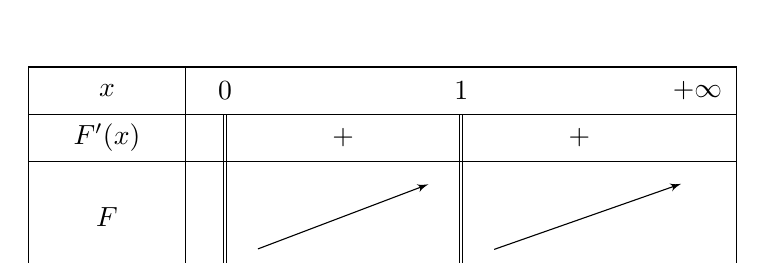
\begin{tikzpicture}
            \tkzTabInit[espcl=3]{$x$/0.6,$F'(x)$/0.6,$F$/1.4}{$0$,$1$,$+\infty$}
            \tkzTabLine{d,+,d,+}
            \tkzTabVar{D-/,+D-/,+/}
        \end{tikzpicture}
    \end{center}
    \boxed{3.} \textbf{Limite en $+\infty$:} Soit $x>1$. $\forall t\in[x,x^2] ~ \frac{1}{\ln(t)}\geq\frac{1}{\ln(x^2)}$ alors par croissance de l'intégrale ($x<x^2$):
    \begin{equation*}
        \int_x^{x^2}\frac{1}{\ln t}\dt\geq\int_x^{x^2}\frac{1}{\ln x^2}\dt \text{ donc } F(x)\geq\frac{x(x-1)}{2\ln(x)}\to+\infty
    \end{equation*}
    Par minoration, $F(x)\to+\infty$ en $+\infty$.\n
    \textbf{Limite en $0_+$:} On encadre pour $x\in]0,1[$ : $\frac{1}{\ln(x)}\leq\frac{1}{\ln(t)}\leq\frac{1}{\ln(x^2)}$ alors ($x^2<x$):
    \begin{equation*}
        \int_x^{x^2}\frac{1}{\ln(x)}\dt\geq\int_x^{x^2}\frac{1}{\ln t}\dt\geq\int_x^{x^2}\frac{1}{\ln(x^2)}\dt
    \end{equation*}
    Donc $\frac{x(x-1)}{2\ln(x)} \leq F(x)\leq \frac{x(x-1)}{\ln(x)}$ Par encadrement, $F(x)\to0$ en $0_+$.\n
    \textbf{Limite en $1_+$:}Pour $x>1$, $F(x)=L(x^2)-L(x)$ et $L'(x)=\frac{1}{\ln(x)}\sim_1\frac{1}{x-1}$ donc $L'(x)=_1\frac{1}{x-1}+o(\frac{1}{x-1})$.\\
    Posons $R(x)=L'(x)-\frac{1}{x-1}$ continue sur $]1,+\infty[$.\\
    On a :
    \begin{align*}
        F(x)&=\int_x^{x^2}L(t)\dt=\int_x^{x^2}\left(\frac{1}{t-1}+R(t)\right)\dt=\int_x^{x^2}\frac{1}{t-1}\dt+\int_x^{x^2}R(t)\dt\\
        \int_x^{x^2}\frac{1}{t-1}\dt&=\ln(x^2-1)-\ln(x-1)=\ln(x+1)\xrightarrow[x\to1_+]{}\ln(2)
    \end{align*}
    Montrons que $\int_x^{x^2}R(t)\dt\to0$.\\
    On a $(t-1)R(t)\to0$ quand $t\to1_+$.\\
    Soit $\e>0, \exists\eta>0~\forall t\in]1,1+\eta[ ~ -\e\leq(t-1)R(t)\leq\e$ donc $-\frac{\e}{t-1}\leq R(t) \leq \frac{\e}{t-1}$.\\
    Supposons $x\in]1,\sqrt{1+\eta}[$ alors $[x,x^2]\subset]1,1+\eta[$.\\
    Alors $\forall t \in [x,x^2], ~ -\frac{\e}{t-1}\leq R(t) \leq \frac{\e}{t-1}$.\\
    On intégre :
    \begin{equation*}
        -\e\leq-\e\ln(x+1) \leq \int_x^{x^2}R(t)\dt\leq \e\ln(x+1)\leq\e
    \end{equation*}
    On a donc bien $\int_x^{x^2}R(t)\dt=_1o(1)$.\\
    On a donc prouvé que $F(x)=_1\ln(x+1)+o(1)$ donc $F(x)\xrightarrow[x\to1_+]{}\ln2$\n
    \textbf{Limite en $1_-$:} Soit $x\in]0,1[$. On a $F(x)=\int_x^{x^2}t\frac{1}{t\ln t}\dt$. On a $0<x^2<x<1$. Soit $t\in[x^2,x]$.\\
    On a $\frac{x}{t\ln t}\leq t\frac{1}{t\ln t}\leq \frac{x^2}{t\ln t}$. On intégre : $\int_x^{x^2}\frac{x^2}{t\ln t}\dt\leq\int_x^{x^2}\frac{1}{\ln t}\dt \leq \int_x^{x^2}\frac{x}{t\ln t}\dt$.\\
    Or, $\int_x^{x^2}\frac{1}{t\ln t}\dt = \left[ \ln | \ln t | \right]_x^{x^2}=\ln|\ln(x^2)|-\ln|\ln(x)|=\ln(-2\ln(x))-\ln(\ln(-x))=\ln(2)$.\\
    Finalement, $x^2\ln(2)\leq F(x) \leq x\ln(2)$ et par théorème des gendarmes, $F(x)\xrightarrow[x\to1_-]{}\ln(2)$.
\end{ex}

\subsection{Outils de calcul intégral.}

\begin{thm}{Intégration par parties.}{}
    Soient $u,v\in\m{C}^1(I,\K)$ et $a,b\in I$. Alors,
    \begin{equation*}
        \int_a^bu'v=[uv]_a^b-\int_a^buv'.
    \end{equation*}
    \tcblower
    On a $uv$ dérivable comme produit de fonctions dérivables sur $I$.\\
    Alors $(uv)'=u'v + uv'$. Or $u,v$ étant de classe $\m{C}^1$, $u'v$ et $uv'$ sont continues sur $I$.
    \begin{align*}
        \int_a^b(uv)'(t)\dt&=\int_a^b(u'(t)v(t)+u(t)v'(t))\dt\\
        [uv]_a^b &= \int_a^bu'v+\int_a^buv'
    \end{align*}
\end{thm}

\begin{ex}{Suites dont le terme général est une intégrale.}{}
    Soit $(f_n)_{n\in\N}$ une suite de fonctions continues sur $[a,b]$ et $(I_n)_{n\in\N}$:
    \begin{equation*}
        \forall n\in\N ~ I_n := \int_a^bf_n(x)\dx 
    \end{equation*}
    On peut obtenir une relation de récurrence sur la suite $(I_n)$ avec une IPP dans certains cas.
\end{ex}

\begin{thm}{Formule du changement de variable}{}
    Soit $\phi\in\m{DM}^1(I,J)$, $f\in\m{CM}(J,\K)$ et $a,b\in I$. Alors,
    \begin{equation*}
        \int_{\phi(a)}^{\phi(b)}f(t)\dt=\int_a^bf(\phi(x))\phi'(x)\dx
    \end{equation*}
\end{thm}

\begin{ex}{}{}
    En posant $t=\tan\frac{x}{2}$, montrer que: \begin{equation*}\int_{-\frac{\pi}{2}}^{\frac{\pi}{2}}\frac{\dx}{4+\sin x}=\frac{\pi}{\sqrt{15}}\end{equation*} 
    \tcblower
    On pose le changement de variable :
    \begin{center}
        \begin{tabular}{|c|c|c|c|c|}
            \hline
            $t$ & $\dt$ & $\frac{2}{1+t^2}\dt$ & $t=-1$ & $t=1$\\
            \hline
            $\tan\frac{x}{2}$ & $\frac{1}{2}(1+\tan^2(\frac{x}{2}))\dx$ & $\dx$ & $x=-\frac{\pi}{2}$ & $x=\frac{\pi}{2}$\\
            \hline
        \end{tabular}
    \end{center}
    Alors :
    \begin{align*}
        \int_{-\frac{\pi}{2}}^{\frac{\pi}{2}}\frac{\dx}{4+\sin x}&=\int_{-1}^1\frac{1}{4+\frac{2t}{1+t^2}}\cdot\frac{2}{1+t^2}\dt\\
        &=\int_{-1}^1\frac{2}{4t^2+2t+4}\dt
        =\int_{-1}^1\frac{1}{2t^2+t+2}\dt
    \end{align*}
    Pas de racine réelles. On a $2t^2+t+2=2(t^2+\frac{1}{2}+1)=2((t+\frac{1}{4})^2-(\frac{\sqrt{15}}{4})^2)$.\\
    Cours : $\frac{1}{x^2+a^2}=\frac{d}{\dx}(\frac{1}{a}\arctan(\frac{1}{a}))$.\\
    Donc :
    \begin{align*}
        \frac{1}{2}\int_{-1}^1\frac{1}{(t+\frac{1}{4})^2+(\frac{\sqrt{15}}{4})^2}\dt &= \frac{4}{2\sqrt{15}}\left[ \arctan(\frac{4}{\sqrt{15}(t+\frac{1}{4})})\right]_{-1}^1 = \frac{2}{\sqrt{15}}\left[ \arctan(\frac{5}{\sqrt{15}}) + \arctan(\frac{3}{\sqrt{15}}) \right]
    \end{align*}
    Or $\frac{5}{\sqrt{15}}\cdot\frac{3}{\sqrt{15}}=\frac{15}{\sqrt{15}^2}=1$ et $\arctan(x)+\arctan(\frac{1}{x})=\begin{cases}\frac{\pi}{2} ~ (x>0)\\-\frac{\pi}{2} ~ (x<0) \end{cases}$\\
    Alors $\int_{-\frac{\pi}{2}}^{\frac{\pi}{2}}\frac{1}{4+\sin x}\dx=\frac{2}{\sqrt{15}}\frac{\pi}{2}=\frac{\pi}{\sqrt{15}}$
\end{ex}

\begin{corr}{Intégrale d'une fonction paire/impaire.}{}
    Soit $f\in\CM([-a,a],\\K)$.\\
    Si $f$ est paire : $\int_{-a}^af(t)\dt=2\int_0^af(t)\dt$.\\
    Si $f$ est impaire : $\int_{-a}^af(t)\dt=0$.
\end{corr}

\begin{corr}{}{}
    Soit $f\in\CM(\R,\K)$ une fonction $T$-périodique avec $T\in\R^*_+$.
    \begin{equation*}
        \forall a\in\R, ~ \int_a^{a+T}f(t)\dt=\int_0^Tf(t)\dt.
    \end{equation*}
\end{corr}

\begin{thm}{Formule de Taylor avec reste intégral}{}
    Soit $f\in\m{C}^{n+1}([a,b],\K)$ et $x\in[a,b]$. Alors,
    \begin{equation*}
        f(x)=\sum_{k=0}^n\frac{f^{(k)}(a)}{k!}(x-a)^k+\int_a^b\frac{(x-t)^n}{n!}f^{(n+1)}(t)\dt
    \end{equation*}
    \tcblower
    Par récurrence :\\
    \textbf{Cas de base:} Soit $f\in\m{C}^1(I,\K)$ et $a,x\in I$. Alors :
    \begin{equation*}
        f(x)-\sum_{k=0}^0\frac{f^{(k)}(a)}{k!}(x-a)^k=f(x)-f(a)
    \end{equation*}
    Et
    \begin{equation*}
        \int_a^x\frac{(x-t)^0}{0!}f'(t)\dt=\int_a^xf'(t)\dt=f(x)-f(a)
    \end{equation*}
    Le résultat est vrai.\\
    $\textbf{Hérédité:}$ Soit $n\in\N$. Supposons le résultat vrai pour cet entier. Soit $f\in\m{C}^{n+2}(I,\K)$ et $x,a\in I$.\\
    Or $\m{C}^{n+2}(I,\K)\subset\m{C}^{n+1}(I,\K)$, par hypothèse : $f(x)=\sum_{k=0}^n\frac{f^{(k)}(a)}{k!}(x-a)^k+R_n(x)$.\\
    Avec IPP, fonctions de classes $\m{C}^1$, $f^{n+1}$ et $-\frac{(x-t)^{n+1}}{(n+1)!}$ :
    \begin{align*}
        R_n(x)&= \int_a^x\frac{(x-a)^n}{n!}f^{(n+1)}(t)\dt = \left[ -\frac{(x-t)^{n+1}}{(n+1)!}f^{n+1}(t) \right]_a^x - \int_a^x-\frac{(x-t)^{n+1}}{(n+1)!}f^{n+2}(t)\dt\\
        &=--\frac{(x-a)^{n+1}}{(n+1)!}f^{n+1}(a)+\int_a^x\frac{(x-t)^{n+1}}{(n+1)!}f^{n+2}(t)\dt
    \end{align*}
    Bilan : $f(x)=\sum_{k=0}^{n+1}\frac{f^{(k)}(a)}{k!}(x-a)^k+\int_a^x\frac{(x-t)^{n+1}}{(n+1)!}f^{(n+2)}(t)\dt$\\
    L'identité est vraie au rang $n+1$ donc vraie pour tout $n$ par récurrence.
\end{thm}

\begin{ex}{Comparer une fonction et son polynôme de Taylor}{}
    Montrer l'inégalité :
    \begin{equation*}
        \forall x \in \left[ 0,\frac{\pi}{2} \right], \quad \cos x \geq 1 - \frac{x^2}{2!}.
    \end{equation*}
    \tcblower
    On a $\cos$ de classe $\m{C}^{\infty}$ donc $\m{C}^3$ sur $[0, \frac{\pi}{2}]$ donc d'après Taylor avec Reste intégral :
    \begin{equation*}
        \cos(x) = x - \frac{x^2}{2!} + \int_0^x\frac{(x-t)^2}{2!}\cos^{(3)}(t)\dt
    \end{equation*}
    Donc $\cos(x) - x + \frac{x^2}{2!} = \int_0^x\frac{(x-t)^2}{2!}\sin(t)\dt$. Cette intégrale est positive car continue, positive et $0\leq x$.\\
    On en déduit bien l'inégalité.
\end{ex}

\begin{prop}{Inégalité de Taylor-Lagrange}{}
    Soit $I$ un intervalle, $a\in I$, $n\in \N$ et $f\in\m{C}^{n+1}(I,\K)$.\\
    On suppose que la fonction $|f^{(n+1)}|$ est majorée par une constante $M_{n+1}$ sur $I$. Alors
    \begin{equation*}
        \forall x \in I, ~ \Big|f(x)-\sum_{k=0}^n\frac{f^{(k)}(a)}{k!}(x-a)^k\Big|\leq M_{n+1}\frac{|x-a|^{n+1}}{(n+1)!}
    \end{equation*}
    \tcblower
    D'après Taylor avec reste intégral, $\min:=\min(a,x)$ et $\max:=\max(a,x)$ :
    \begin{equation*}
        \Big|f(x)-\sum_{k=0}^n\frac{f^{(k)}(a)}{k!}(x-a)^k\Big|=\Big|\int_a^x\frac{(x-t)^n}{n!}f^{(n+1)}(t)\dt\Big|\leq\int_{\min}^{\max}\frac{|x-t|^n}{n!}|f^{n+1}(t)|\dt
    \end{equation*}
    Par croissance de l'intégrale, $\int_{\min}^{\max}\frac{|x-t|^n}{n!}|f^{n+1}(t)|\dt\leq\int_{\min}^{\max}\frac{|x-t|^n}{n!}M_{n+1}\dt=\frac{M_{n+1}}{(n+1)!}|x-a|^{n+1}$
\end{prop}

\begin{ex}{}{}
    Prouver que 
    \begin{equation*}
        \forall x \in [0,1], ~ \lim_{n\to+\infty}\sum_{k=1}^n\frac{(-1)^{k-1}}{k}x^k=\ln(1+x).
    \end{equation*}
    \tcblower
    Soit $x\in[0,1]$ et $\forall k\in\N^*, ~ u_k = \frac{x^k}{k}$ décroissante vers 0.\\
    La série $\sum(-1)^ku_k$ converge (thm des séries alternées.).\\
    Notons $f:x\mapsto\ln(1+x)$. Posons $n\in\N^*$ et $T_n$ son polynome de Taylor à l'ordre $n$ en 0.
    \begin{equation*}
        T_n = \sum_{k=1}^n\frac{f^{(k)}(0)}{k!}X^k=\sum_{k=1}^n\frac{(-1)^k}{k}X^k
    \end{equation*}
    On majore $|f-T_n|$ avec Taylor-Lagrange. On a $f^{(n+1)}(x)=\frac{(-1)^n(n)!}{(1+x)^{n+1}}$ majorée par $n!$ sur $[0,1]$.\\
    Donc l'inégalité donne :
    \begin{equation*}
        |f(x)-T_n(x)|\leq n!\frac{|x|^{n+1}}{(n+1!)}\leq\frac{1}{n+1}
    \end{equation*}
    Par encadrement, $T_n(x)\xrightarrow[n\to+\infty]{} f(x)$.
\end{ex}

\section{Sommes de Riemann}
\subsection{Convergence des sommes de Riemann}

\begin{defi}{}{}
    Soit un segment $[a,b]$ avec $a<b$. Pour $n\in\N^*$ et $k\in\lb0,n\rb$, on note $a_k=a+k\frac{b-a}{n}$.\\
    La famille $(a_0,...,a_n)$ est appelée subdivision régulière de $[a,b]$ à $n$ segments. Chaque segment de la subdivision est de longueur $\frac{b-a}{n}$, et ce nombre est appelé pas de la subdivision.\\
    Soit $f\in\CM([a,b], \K)$. On appelle $n$ème somme de Riemann de $f$ le nombre
    \begin{equation*}
        R_n(f)=\frac{b-a}{n}\sum_{k=0}^{n-1}f(a_k)
    \end{equation*}
\end{defi}

\begin{thm}{Convergence des sommes de Riemann}{}
    Soit $f\in\CM([a,b], \K)$.\\
    Pour $n\in\N^*$ et $k\in\lb0,n\rb$, on note $a_k=a+k\frac{b-a}{n}$ et $R_n(f)=\frac{b-a}{n}\sum_{k=0}^{n-1}f(a_k)$. Alors,
    \begin{equation*}
        R_n(f)\xrightarrow[n\to+\infty]{}\int_a^bf(t)\dt
    \end{equation*}
    \tcblower
    \textbf{Remarque:} on écrira la preuve dans le cas $f$ lipschitzienne.
\end{thm}

\begin{corr}{Cas particulier important}{}
    Soit $f\in\CM([0,1], \K)$.
    \begin{equation*}
        \frac{1}{n}\sum_{k=0}^{n-1}f\left(\frac{k}{n}\right)\xrightarrow[n\to+\infty]{}\int_0^1f(t)\dt
    \end{equation*}
    \tcblower
    C'est le théorème avec $a=0$ et $b=1$.
\end{corr}

\begin{ex}{}{}
    Calculer :
    \begin{equation*}
        \lim\frac{1}{n}\sum_{k=1}^n\frac{\sqrt{k}}{\sqrt{n}} \quad \text{et}  \quad \lim\sum_{k=0}^{n-1}\frac{1}{n+k}
    \end{equation*}
    \tcblower
    Posons $f:x\mapsto\sqrt{x}$, on a $\frac{1}{n}\sum_{k=1}^n\frac{\sqrt{k}}{\sqrt{n}}$.\\
    On a $f$ continue, c'est une somme de Riemann, par convergence des sommes de Riemann:
    \begin{equation*}
        \frac{1}{n}\sum_{k=1}^n\frac{\sqrt{k}}{\sqrt{n}}\to\int_0^1\sqrt{t}\dt=\left[ \frac{2}{3}x^{3/2} \right]_0^1=\frac{2}{3}.
    \end{equation*}
    Posons $g:x\mapsto\frac{1}{1+x}$. On a $g$ continue, c'est une somme de Riemann, par converge :
    \begin{equation*}
        \sum_{k=0}^{n-1}\frac{1}{n+k}\to\int_0^1\frac{1}{1+t}\dt=\left[ \ln|1+t| \right]_0^1=\ln2
    \end{equation*}
\end{ex}

\begin{ex}{Inégalité de Jensen pour les intégrales}{}
    \textcolor{red}{\textbf{CENTRALE 2024}}\\
    Soit $f:[a,b]\to\R$ une fonction CPM à valeurs dans $I$ et $\phi$ une fonction convexe et continue sur $I$.\\
    Démontrer l'inégalité de Jensen pour les intégrales :
    \begin{equation*}
        \phi\left(\frac{1}{b-a}\int_a^bf(t)\dt\right) \leq \frac{1}{b-a}\int_a^b\phi(f(t))\dt
    \end{equation*}
    \tcblower
    On sait (CV des sommes de Riemann) :
    \begin{equation*}
        \frac{1}{b-a}\int_a^bf(t)\dt=\lim_{n\to+\infty}\frac{1}{n}\sum_{k=0}^{n-1}f(a_k)
    \end{equation*}
    On a $\phi$ convexe sur $I$, on pose $\l_i=\frac{1}{n}$ et $x_i=f(a_i)$ pour $i\in\lb1,n\rb$.\\
    D'après l'inégalité de Jensen :
    \begin{equation*}
        \phi\left(\frac{1}{n}\sum_{i=1}^nf(a_i)\right)\leq\frac{1}{n}\sum_{i=1}^n\phi(f(a_i))
    \end{equation*}
    Donc, puisque $\phi$ est $\CM$ sur $[a,b]$
    \begin{equation*}
        \frac{1}{n}\sum_{i=1}^n\phi\circ f(a_i) \xrightarrow[n\to+\infty]{}\frac{1}{b-1}\int_a^b\phi\circ f(t)\dt
    \end{equation*}
    D'après le théorème sur les sommes de $\R$.\\
    De même, $\frac{1}{n}\sum_{i=1}^nf(a_i)\xrightarrow[n\to+\infty]{}\frac{1}{b-a}\int_a^bf(t)\dt$.\\
    On a bien $\phi\left(\frac{1}{n}\sum_{i=1}^nf(a_i)\right)\to\phi\left(\frac{1}{b-a}\int_a^bf(t)\dt\right)$ lorsque $I=\R$.\\
    Par stabilité des inégalités larges :
    \begin{equation*}
        \phi\left(\frac{1}{b-a}\int_a^bf(t)\dt\right)\leq\frac{1}{b-a}\int_a^b\phi\circ f(t)\dt
    \end{equation*}
\end{ex}

\pagebreak

\subsection{Comparaison de la méthode des rectangle avec celle des trapèzes.}

\begin{prop}{Erreur d'approximation avec la méthode des rectangles}{}
    Soit $f:[a,b]\to\K$ une fonction $M$-lipschitzienne, avec $M\in\R^*_+$.\\
    Notons $R_n(f)=\frac{b-a}{n}\sum_{k=0}^{n-1}f(a+k\frac{b-a}{k})$, pour tout $n\in\N^*$.\\
    Ce nombre est une valeur approchée de l'intégrale de $f$ entre $a$ et $b$.\\
    Voici une majoration de l'erreur : $\Big|R_n(f)-\int_a^bf(t)\dt\Big|\leq\frac{M(b-a)^2}{2n}$.\\
    On a donc $\Big|R_n(f)-\int_a^bf(t)\dt\Big|=O(\frac{1}{n})$.
    \tcblower
    On a :
    \begin{align*}
        \Big|R_n(f)-\int_a^bf\Big| &= \Big|\frac{b-a}{n}\sum_{k=0}^{n-1}f(a_k)-\sum^{n-1}_{k=0}\int_{a_k}^{a_{k+1}}f\Big|\\
        &= \Big|\sum_{k=0}^{n-1}\left( \frac{b-a}{n}f(a_k) - \int_{a_k}^{a_{k+1}}f(t)\dt \right)\Big|\\
        &=\Big|\sum_{k=0}^{n-1}\left(\int_{a_k}^{a_{k+1}}f(a_k)\dt-\int_{a_k}^{a_{k+1}}f(t)\dt\right)\Big|\\
        &=\Big|\sum_{k=0}^{n-1}\int_{a_k}^{a_{k+1}}\left(f(a_k)-f(t)\right)\dt\Big|\\
        &\leq \sum_{k=0}^{n-1}\int_{a_k}^{a_{k+1}}\Big|f(a_k)-f(t)\Big|\dt
    \end{align*}
    Pour $k$ fixé, $\forall t \in [a_k,a_{k+1}], ~ |f(a_k)-f(t)|\leq M(b-a_k)$.\\
    Par croissance de l'intégrale :
    \begin{equation*}
        \int_{a_k}^{a_{k+1}}\Big|f(a_k)-f(t)\Big|\dt\leq M\int_{a_k}^{a_{k+1}}(t-a_k)\dt\leq \frac{1}{2}M(a_{k+1}-a_k)^2\leq\frac{M}{2}(\frac{b-a}{2})^2
    \end{equation*}
    On somme :
    \begin{equation*}
        \Big| R_n(f) - \int_a^bf\Big| \leq \sum_{k=0}^{n-1}\frac{M}{2}\frac{(b-a)^2}{n^2}\leq \frac{M(b-a)^2}{2n}=O(\frac{1}{n})
    \end{equation*}
\end{prop}

\begin{prop}{Erreur d'approximation avec la méthode des trapèzes}{}
   Soit $f\in\m{C}^2([a,b],\K)$. Pour $n\in\N^*$, on définit $T_n(f)$ comme :
   \begin{equation*}
        T_n(f):=R_n(f)+\frac{b-a}{n}\cdot\frac{f(b)-f(a)}{2}
   \end{equation*}
   Alors :
   \begin{equation*}
    \Big|T_n(f)-\int_a^bf(t)\dt\Big|=O\left(\frac{1}{n^2}\right)
   \end{equation*}
\end{prop}

\subsection{Complément : continuité uniforme d'une fonction.}

\begin{defi}{Uniforme continuité}{}
    Soit une fonction $f:I\to\K$. On dit que $f$ est uniformément continue sur $I$ si:
    \begin{equation*}
        \forall \e>0, ~ \exists \eta > 0 ~ \forall (x,y) \in I^2, ~ |x-y|\leq\eta \Longrightarrow |f(x)-f(y)|\leq\e.
    \end{equation*}
\end{defi}

\begin{prop}{}{}
    Toute fonction lipschitzienne sur un intervalle $I$ y est uniformément continue.
    \tcblower
    Soit $f:I\to\K$ on suppose qu'il existe $K>0$ telle que $\forall x,y\in I^2, ~ |f(x)-f(y)|\leq K|x-y|$.\\
    Soit $\e>0$, on pose $\eta=\frac{\e}{K}$. Soit $(x,y)\in I^2 ~ | ~ |x-y|\leq\eta$ alors $f|(x)-f(y)|\leq K|x-y| \leq K\eta = \e$.
\end{prop}

\begin{thm}{de Heine}{}
    Toute fonction continue sur un segment y est uniformément continue.
    \tcblower
    Par l'absurde, soit $f:I\to\K$ continue sur $[a,b]$ mais non uniformément continue.
    \begin{equation*}
        \exists \e > 0, ~ \forall \eta > 0 ~ \exists (x,y)\in I^2, ~ |x-y|\leq\eta \text{ et } |f(x)-f(y)|>\e 
    \end{equation*}
    Soit un tel $\e$. Pour $n\in\N^*, ~ \exists(x_n,y_n)\in I^2 ~ |x_n-y_n| \leq \frac{1}{n}$ et $|f(x)-f(y)|>\e$.\\
    D'après le théorème de Bolzano-Weierstrass, puisque $(x_n)$ et $(y_n)$ sont bornées, on peut extraire deux suites convergentes : $\exists \phi:\N\to\N \text{ strictement croissante} \mid x_{\phi(n)}$ converge vers $l\in\R$.\\
    Pour $n\in\N$, $|y_{\phi(n)}-l|=|y_{\phi(n)}-x_{\phi(n)}+x_{\phi(n)}-l|\leq|y_{\phi(n)}-x_{\phi(n)}|+|x_{\phi(n)}-l|$ donc $y_{\phi(n)}\to l$.\\
    On a $\forall n\in\N^*, ~ |f(x_{\phi(n)})-f(y_{\phi(n)}))|>\e$ et $f$ continue en $l\in[a,b]$ donc $f(x_{\phi(n)})\to f(l)$.\\
    De même pour $f(y_{\phi(n)})\to f(l)$. Par passage à la limite, $|f(l)-f(l)|\geq\e$ et $\e\leq0$, absurde.
\end{thm}
\end{document}
